\documentclass[20pt, a0paper, landscape, colspace=10mm, blockverticalspace=10mm]{tikzposter}
\usepackage[sfmath]{kpfonts}
\usepackage[default]{gillius}
\usepackage[backend=biber, style=authoryear, uniquelist=minyear, uniquename=false]{biblatex}
\usepackage{multirow}
\usepackage{capt-of}
\usepackage{adjustbox}
\usepackage{qrcode}
\usepackage{multicol}
\graphicspath{{../figures/}}
\newcommand{\tablepath}{../tables}

\usetheme{Board}
\usetikzlibrary{calc}

\addbibresource{papers.bib}
\setlength{\bibhang}{0pt}
\DeclareBibliographyCategory{ignore}
\addtocategory{ignore}{zetterberg2004two}
\addtocategory{ignore}{niculescu2015recent}
\addtocategory{ignore}{novitsky2013phylogenetic}
\addtocategory{ignore}{novitsky2014impact}
\addtocategory{ignore}{mccormack2002early}
\addtocategory{ignore}{grabowski2014role}
\addtocategory{ignore}{wang2015targeting}
\addtocategory{ignore}{kao2011surveillance}
\addtocategory{ignore}{little2014using}
\addtocategory{ignore}{li2015hiv}
\addtocategory{ignore}{cuevas2009hiv}

\tikzposterlatexaffectionproofoff
\settitle{ \vbox{ \centering \color{titlefgcolor}
{\fontsize{2.5cm}{2cm}\selectfont \@title}
\\ --- \huge \@author~--- \\ \@institute } }

\title{Likelihood-free estimation of contact network parameters from viral phylogenies}
\author{Rosemary M. McCloskey$^1$, Richard H. Liang$^1$, and Art F. Y. Poon $^{1,2}$}
\date{March 11, 2015}
\institute{$^1$ BC Centre for Excellence in HIV/AIDS 
           $^2$ Department of Medicine, University of British Columbia}
\begin{document}

\colorlet{blockbodybgcolor}{white}
\node at (current page.west) 
  [anchor=north] {
  
\includegraphics[width=\paperwidth, trim=0 0 0 1in]{logos/cfe_banner}
};

\maketitle[width=1.2\linewidth]

% hacky things
\node [text width=6in] at ($ (current page.west) + (-0.42\paperwidth, -1.5in) $)
  { \LARGE ISMB \\ July 8-12, 2016 \\ Orlando, USA};
\node [text width=6in, align=right] at ($ (current page.west) + (0.42\paperwidth, -1.5in) $)
  { \LARGE rmccloskey@cfenet.ubc.ca \\ (604) 558-8865 };

\begin{columns}
  \column{0.25}
  \block{Contact networks shape viral transmission trees}{
    \centerline{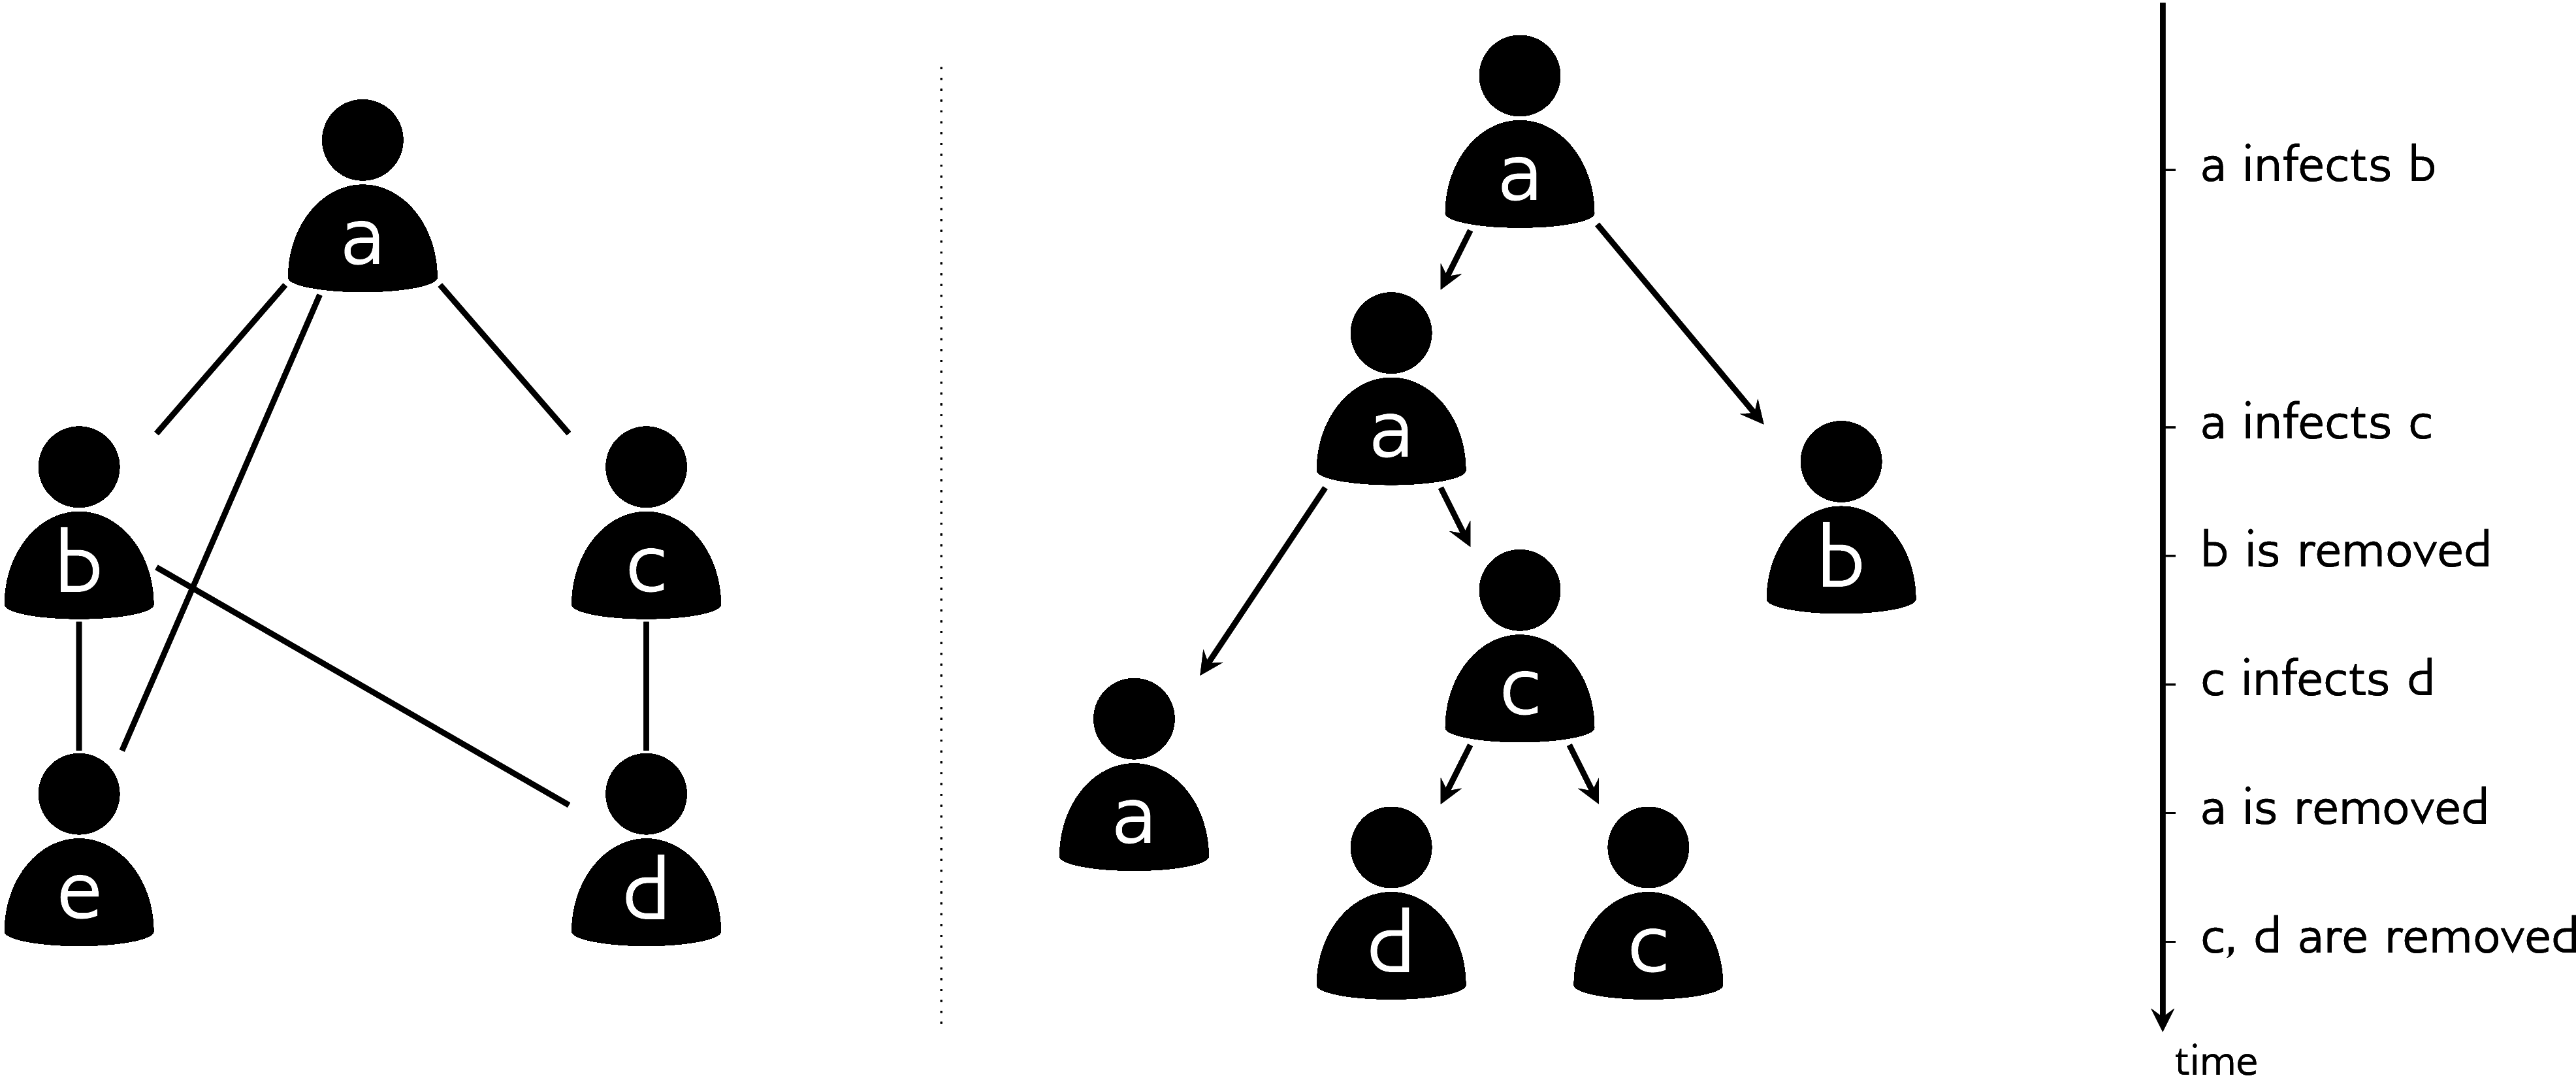
\includegraphics[width=0.22\textwidth]{contactnet}}
      Network structure can change the speed and pattern of epidemic spread,
      potentially informing public health interventions.
  }
  \block{}{\vspace{1cm}\color{blocktitlefgcolor}\bfseries\LARGE{
    \centering
    \centerline{What can we tell about contact}
    
    \centerline{networks from viral sequences?}
  }}

  \block{Barab\'asi-Albert preferential attachment networks}{
    Nodes are added one at a time until there are $N$ total. Each time a node
    is added, $m$ new edges are connected to it. Each new edge is attached to
    an existing node of degree $d$ with probability proportional to
    $d^\alpha + 1$. 

    %\node at (0, 0) {sub-linear $\alpha$};
    %\node at (14, 6.5) {linear $\alpha$};
    %\node at (23, 7.5) {super-linear $\alpha$};

    \begin{center}
      \begin{tikzpicture}
        \node (a) {\includegraphics[width=0.22\textwidth]{pa-example}};
        \node at (a.south) [anchor=north] {sub-linear $\alpha$ $\qquad\qquad\qquad$ linear $\alpha$ $\qquad\qquad\qquad$ super-linear $\alpha$};
      \end{tikzpicture}
    \end{center}

    \begin{center}
      \begin{tabular}{cl}
        parameter & meaning \\
        \hline
        $\alpha$ & preferential attachment power \\
        $m$ & number of new edges added for each new vertex \\
        $I$ & number of infected nodes when epidemic is stopped \\
        $N$ & total number nodes in the network \\
        \hline
      \end{tabular}
    \end{center}
  }

  \block{}{
    \vspace{1.5cm}
    \centerline{\qrcode{https://github.com/rmcclosk/netabc}
    \LARGE{github.com/rmcclosk/netabc}}
  }

  \column{0.225}
  \block{\textit{netabc}: tree kernel + approximate Bayesian computation +
         sequential Monte Carlo}{
    \centerline{\includegraphics[width=0.18\textwidth]{abc-idea}}
    \nocite{del2012adaptive}
    \nocite{poon2013mapping}

    \vspace{1cm}
      ``Particles'' are sampled from prior distributions on model parameters.
      Simulated trees are generated for each particle and compared to the
      observed tree with a phylogenetic kernel~\autocite{poon2013mapping}.
      Particles whose simulated trees are distant from the observed tree are
      removed. Surviving particles are perturbed, and new simulated datasets
      are generated. Iteration leads to an approximation of the posterior
      distribution on the model parameters.
  }

  \block{Varying $\alpha$ and $I$ affects tree shape, but not $m$ and $N$}{
    \centerline{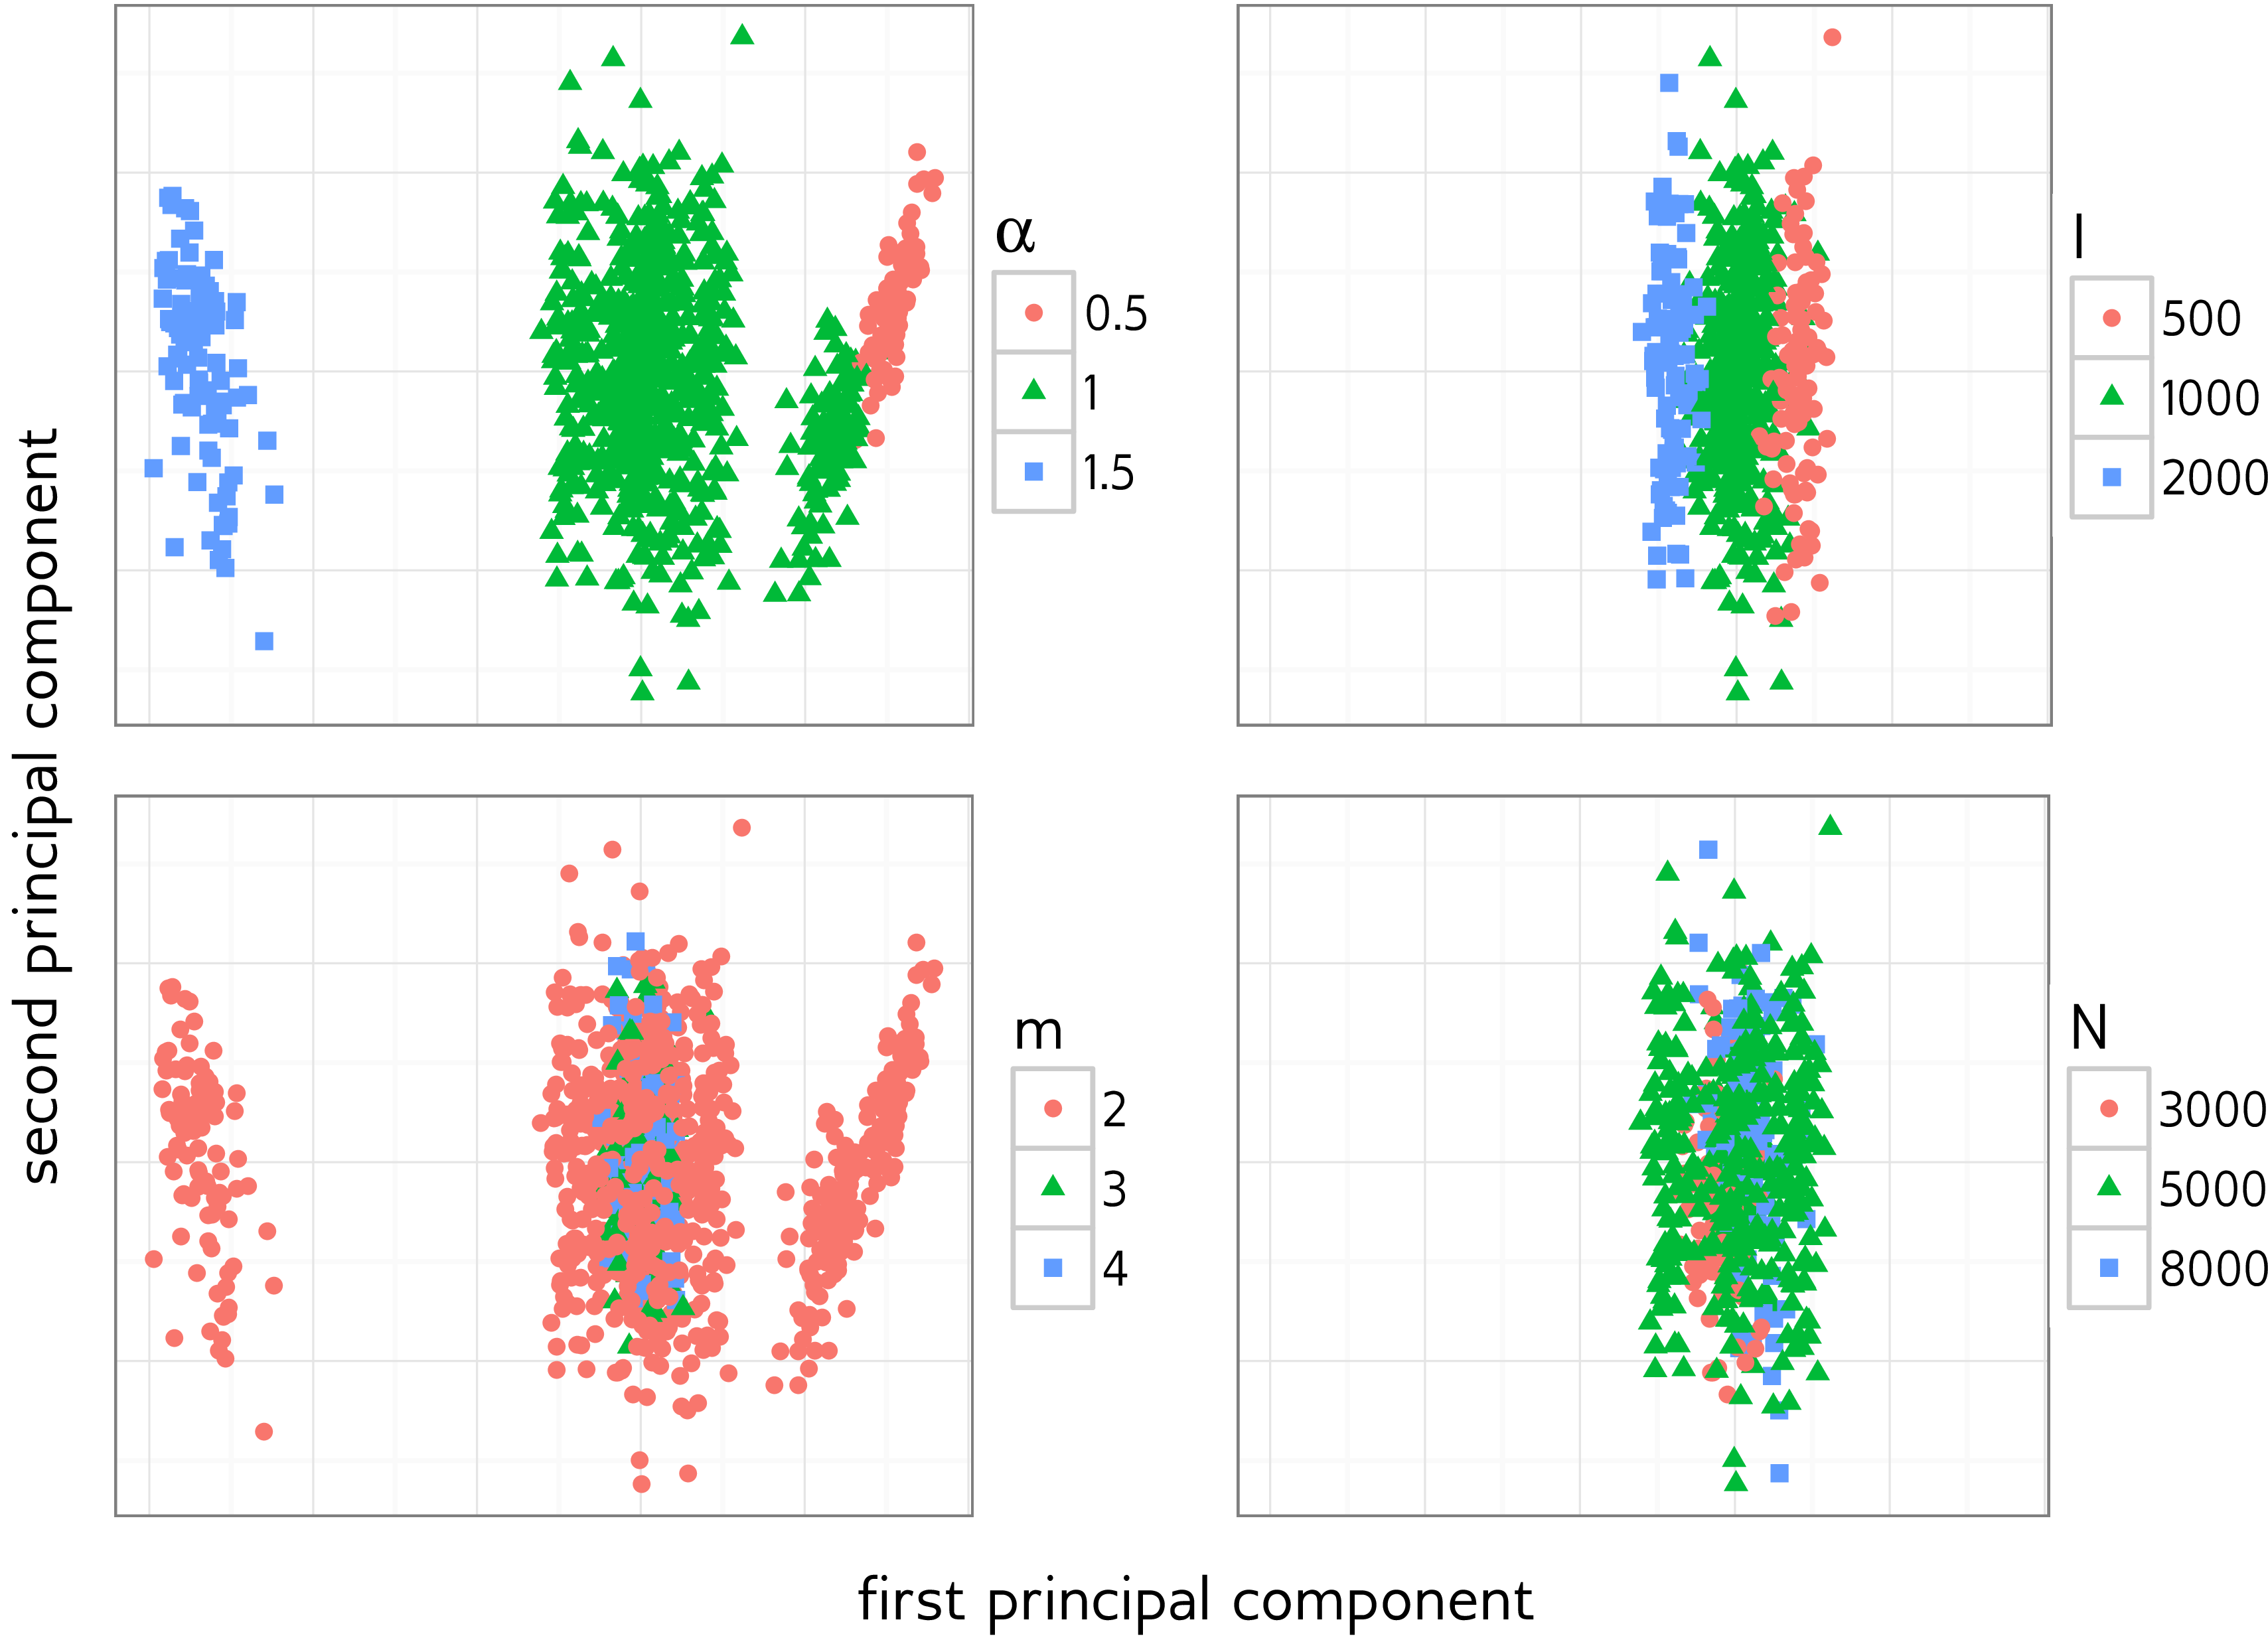
\includegraphics[width=0.16\textwidth]{kernel-kpca}}

      We simulated 100 trees of size 500 under each parameter value. Parameters
      not being tested were fixed at $\alpha$ = 1.0, $m$ = 2, $I$ = 1000, $N$ =
      5000. A $300 \times 300$ kernel matrix of all pairwise similarities was 
      projected onto its first two principal components.
  }

  \column{0.225}
  \block{Simulations}{
    \centering
    \begin{tabular}{ccc}
     parameter & values & prior \\
      \hline
      $\alpha$ & 0.0, 0.5, 1.0, 1.5 & Uniform(0, 2) \\
      $m$ & 2, 3, 4 & Uniform(1, 6) \\
      $I$ & 1000, 2000 & Uniform(500, 5000) \\
      $N$ & 5000 & Uniform(500, 15000) \\
      \hline
    \end{tabular}

    \vspace{0.5cm}
    \captionof{table}{
    Three networks/trees were simulated under each parameter combination.
    Kernel-ABC was used to re-estimate the parameters.
    }
  }
  \block{Accurate estimates for $\alpha$, $I$; not $m$, $N$}{
    \centerline{\includegraphics[width=0.16\textwidth]{abc-point-estimate-m2}}
    Dotted lines are true values. $\alpha$ and $I$, which had the most impact
    on tree shape, were possible to estimate accurately. Posterior
    distributions of $m$ and $N$ heavily resemble the priors, indicating
    little information about these parameters in the trees.
  }
  \block{Narrow dispersion of $\alpha$, $I$ compared to $m$, $N$}{
    \centerline{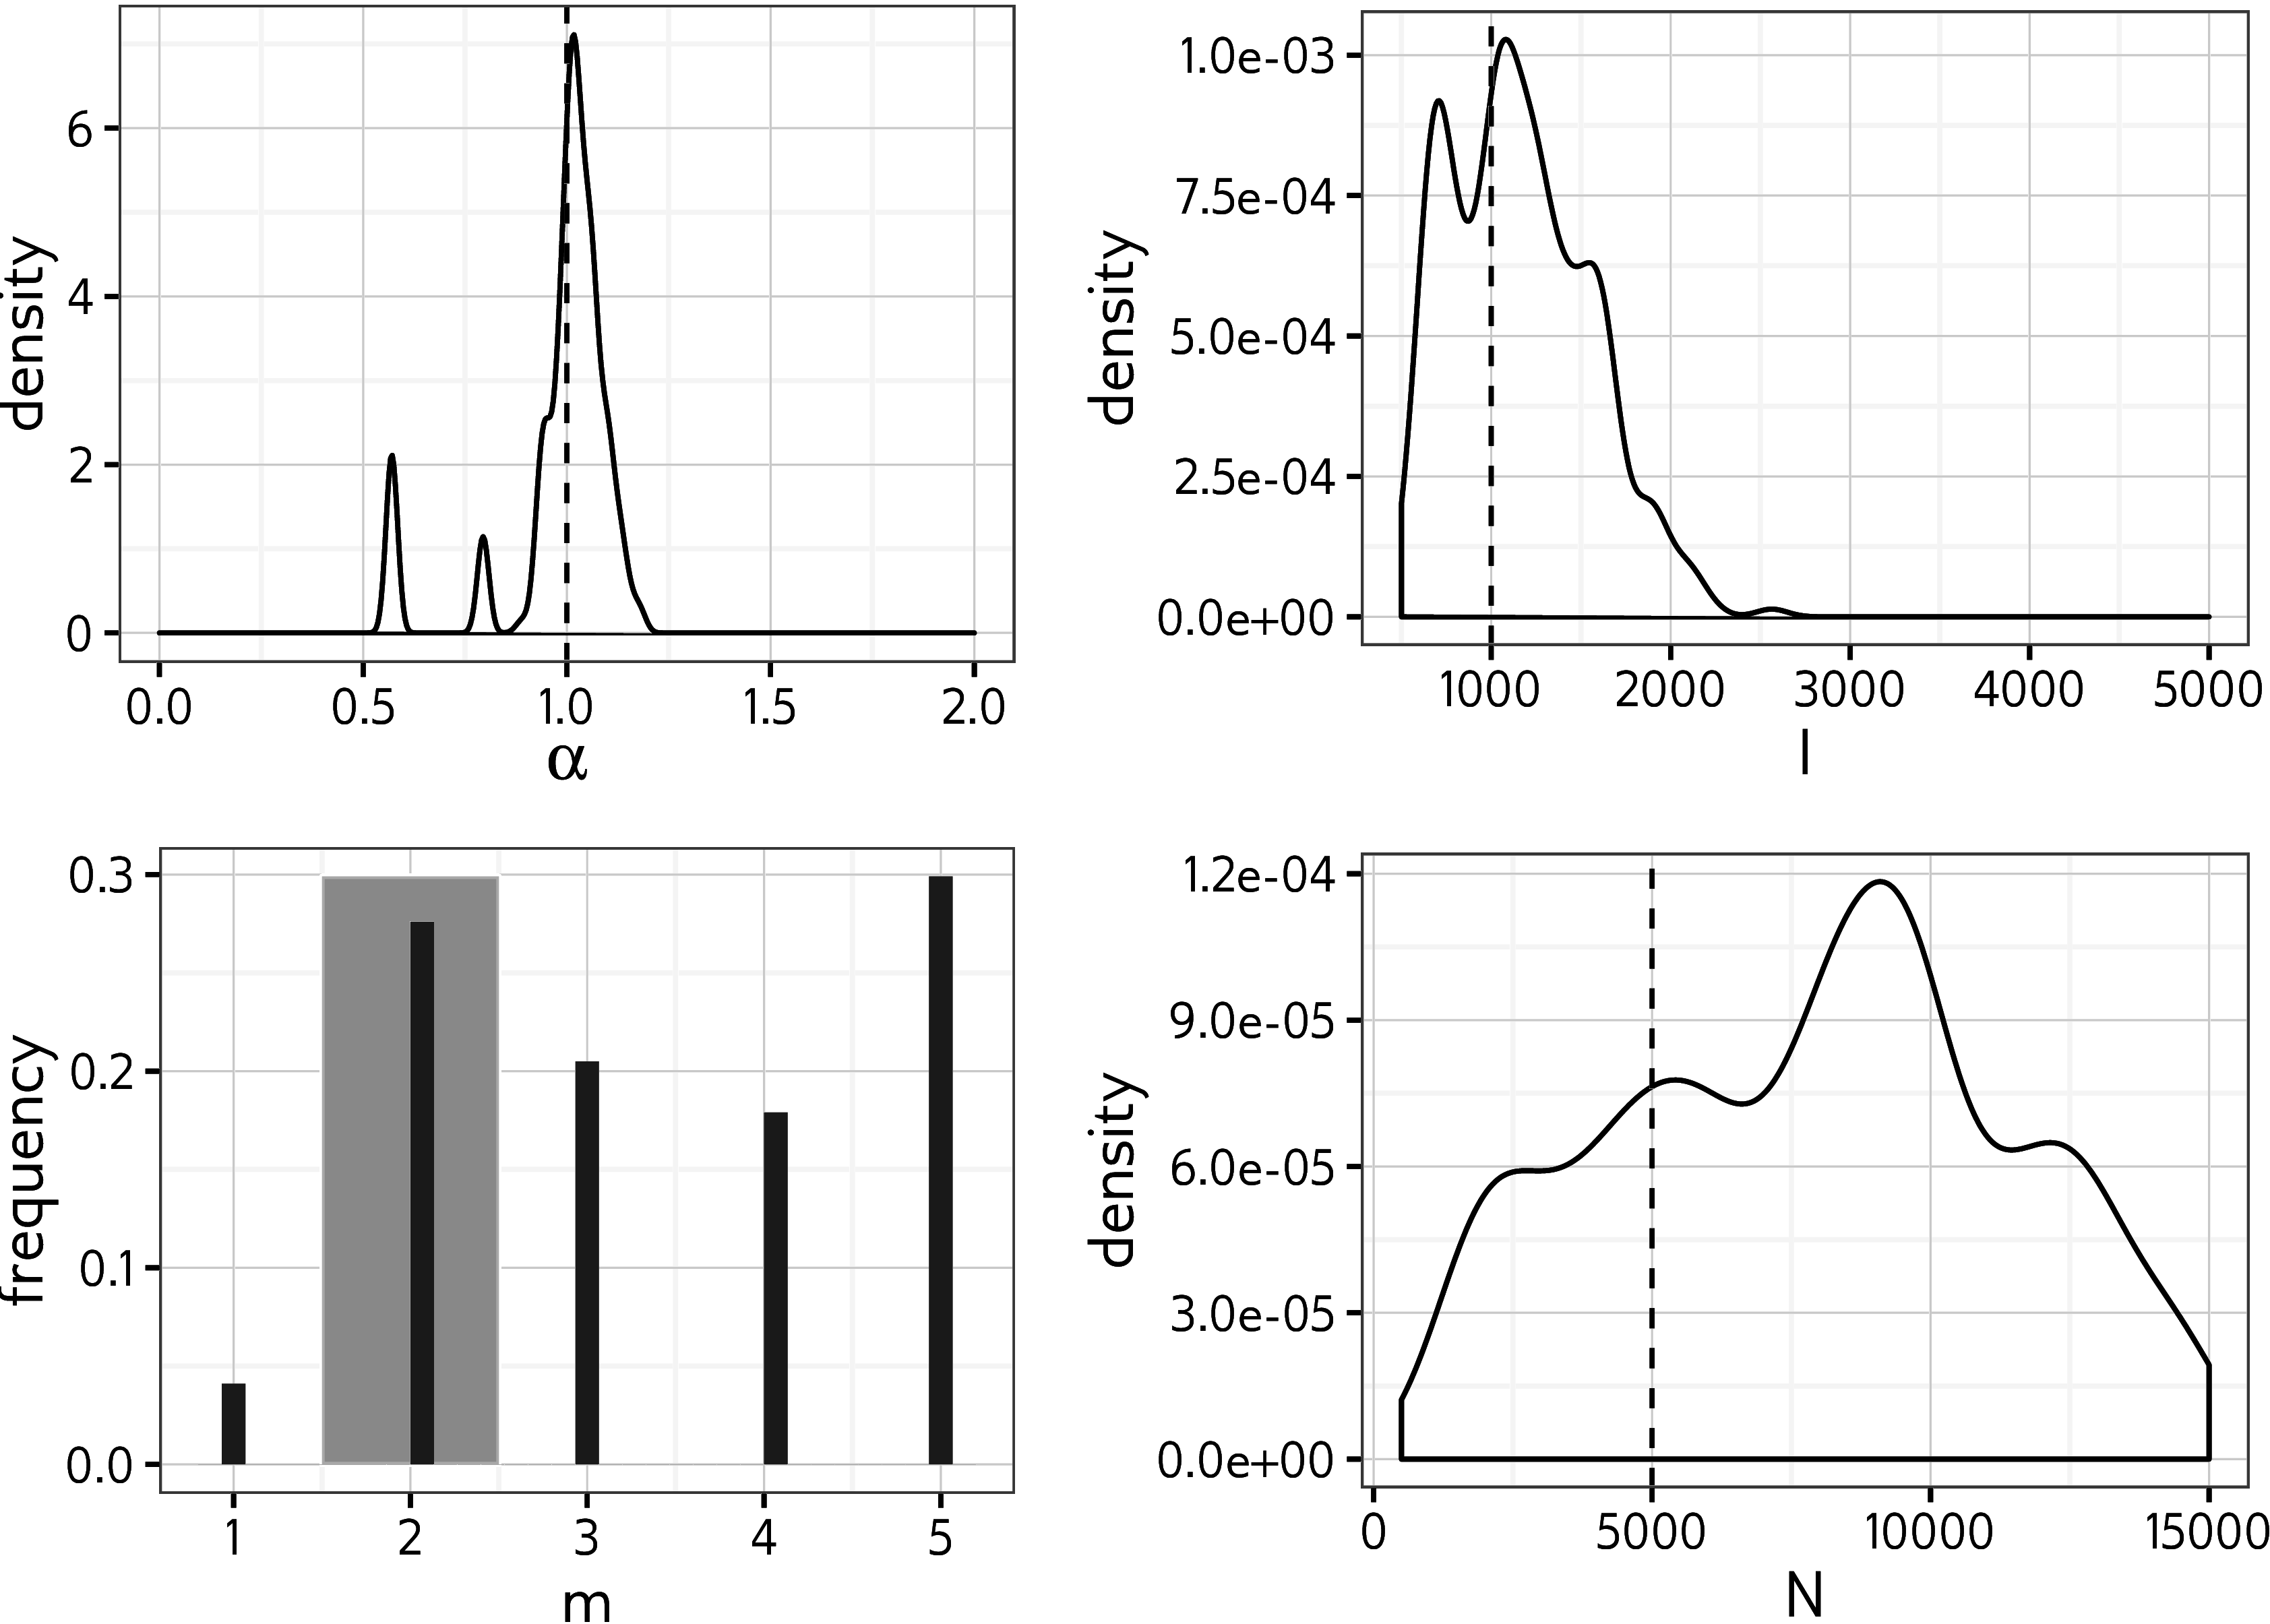
\includegraphics[width=0.15\textwidth]{abc-posterior-example}}
  }

  \column{0.3}

  \block{Real data: phylogenetic and geographic clusters}{
    \centering
    \normalsize
    \begin{tabular}{ccccc}
  Reference & Sequences ($n$) & Location & Risk group & Gene \\
  \hline
  \textcite{wang2015targeting} & 173 & Beijing, China & MSM & \textit{pol} \\
  \textcite{cuevas2009hiv} & 287 & Basque Country, Spain & mixed & \textit{pol} \\
  \textcite{novitsky2013phylogenetic} & \multirow{2}{*}{180} &
  \multirow{2}{*}{Mochudi, Botswana} & \multirow{2}{*}{HET} &
  \multirow{2}{*}{\textit{env}} \\ \textcite{novitsky2014impact} \\
  \textcite{li2015hiv} & 280 & Shanghai, China & MSM & \textit{pol} \\
  \textcite{niculescu2015recent} & 136 & Romania & IDU & \textit{pol} \\
  \hline
\end{tabular}

    \captionof{table}{
      Characteristics of HIV datasets analysed with kernel-ABC. Abbreviations:
      MSM, men who have sex with men; IDU, injection drug users.
    }
  }

  \block{Transmission trees were estimated from viral sequences}{
    \vspace{1cm}
    \centerline{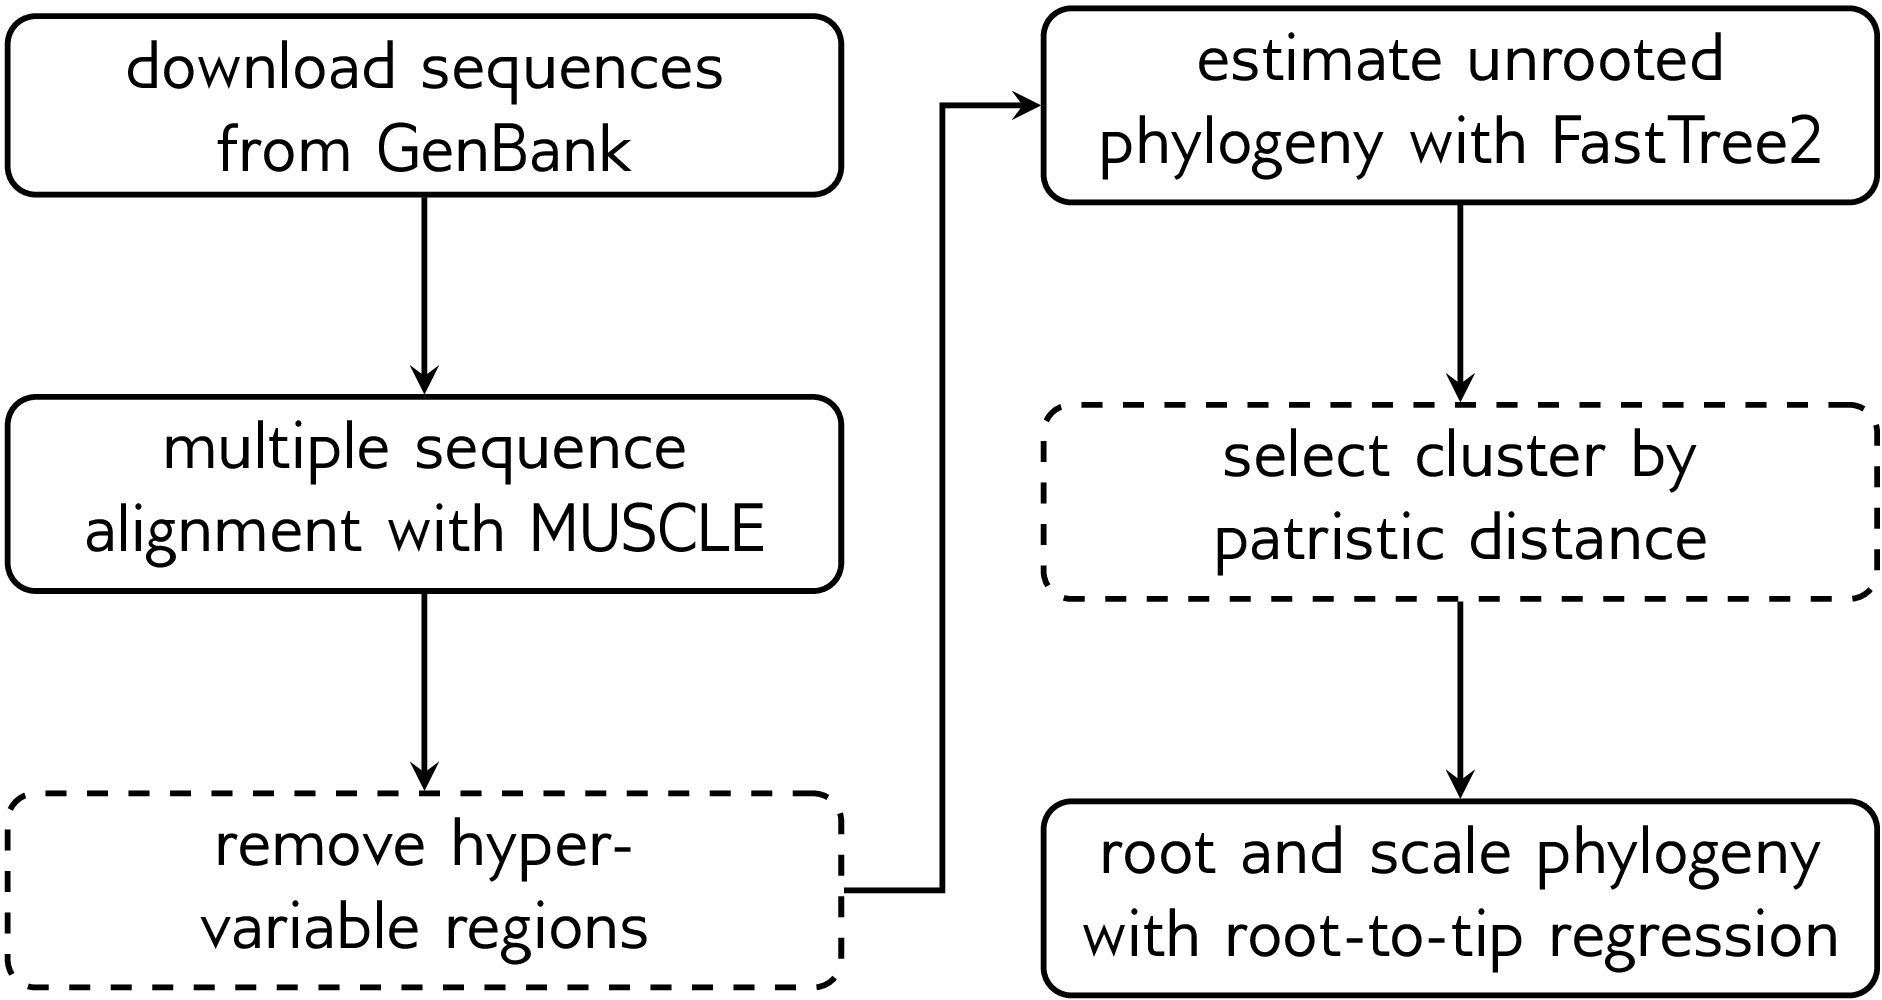
\includegraphics[width=0.25\textwidth]{pipeline}}
    \vspace{1cm}

    \nocite{edgar2004muscle}
    \nocite{price2010fasttree}
    \nocite{drummond2003inference}
  }

  \block{Stronger preferential attachment in IDU networks}{
    \includegraphics[trim=0 3.5in 3.3in 0, clip, width=0.12\textwidth]{realdata-hpd}
    \includegraphics[trim=3.4in 1.5in 0 2.0in, clip, width=0.12\textwidth]{realdata-hpd}
    \vspace{1cm}
  }
\end{columns}

\begin{columns}
  \column{0.65}
  \block{Summary}{
    \setlength{\columnsep}{1cm}
    \begin{multicols}{3}
      We developed a kernel-ABC method for inference of structural contact
      network parameters from viral sequence data. The method is applicable to
      any network model from which networks can be simulated. We demonstrated
      that two of the parameters of the Barab\'asi-Albert preferential
      attachment model can be estimated with kernel-ABC. When applied to real
      data, we observed heterogeneity among model parameters, although
      estimated values of $\alpha$ were consistent with those observed in real
      social networks. 
    
      Due to the simple nature of the Barab\'asi-Albert model, it is likely
      misspecified for the real data we analyzed, and therefore caution must be
      exercised in interpreting the estimated values. However, the possibility
      to investigate more realistic models in the future makes our approach a
      useful tool for phylodynamic research on contact networks.
    \end{multicols}
  }
  \column{0.35}
  \block{References} {
    \renewcommand*{\bibfont}{\footnotesize}
    \printbibliography[notcategory=ignore, heading=none]
    \small
    
\includegraphics[height=1cm]{logos/westgrid} Analyses were run in the
    Westgrid high performance computing environment.
  }
\end{columns}
\block{}{
  \begin{minipage}{0.6\linewidth}
    \vspace{1cm}
    
\includegraphics[width=4in]{logos/btp}
    \quad
    
\includegraphics[width=4in]{logos/cfe}
    \quad
    
\includegraphics[width=2in]{logos/cihr}
    \quad
    
\includegraphics[width=3in]{logos/msfhr}
    \quad
    
\includegraphics[width=3in]{logos/phc}
    \quad
    
\includegraphics[width=1in]{logos/ubc}
    \quad
    
\includegraphics[width=1.8in]{logos/genomecanada}
    \quad
    
\includegraphics[width=2.2in]{logos/genomebc}
    \quad
    
\includegraphics[width=1.8in]{logos/genomequebec}
    \vspace{0.5cm}
  \end{minipage}
  \begin{adjustbox}{valign=t}
    \begin{minipage}[t]{0.4\linewidth}
      \small
      This work was supported by a grant from the Canadian Institutes for
      Health Research (CIHR HOP-111406 to AFYP) and a scholarship from the 
      Canadian Institutes for Health Research  Strategic Training Program in
      Bioinformatics (to RMM). AFYP is the recipient of a Scholar Award from
      the MSFHR/St. Paul’s Hospital Foundation - Providence Health Care
      Research Institute Career Investigator program, and a CIHR New
      Investigator Award.
    \end{minipage}
  \end{adjustbox}
}

\end{document}
